\section{Auswertung}
In diesem Kapitel sollen die aufgenommenen Messwerte Ausgewertet und verrechnet werden.
\subsection{Die statische Methode}
In diesem Kapitel wird die Wärmeleitfähigkeit $\kappa$ von verschiedenen Materialien allein durch die Heizkurve bestimmt.

\begin{figure}
    \centering
    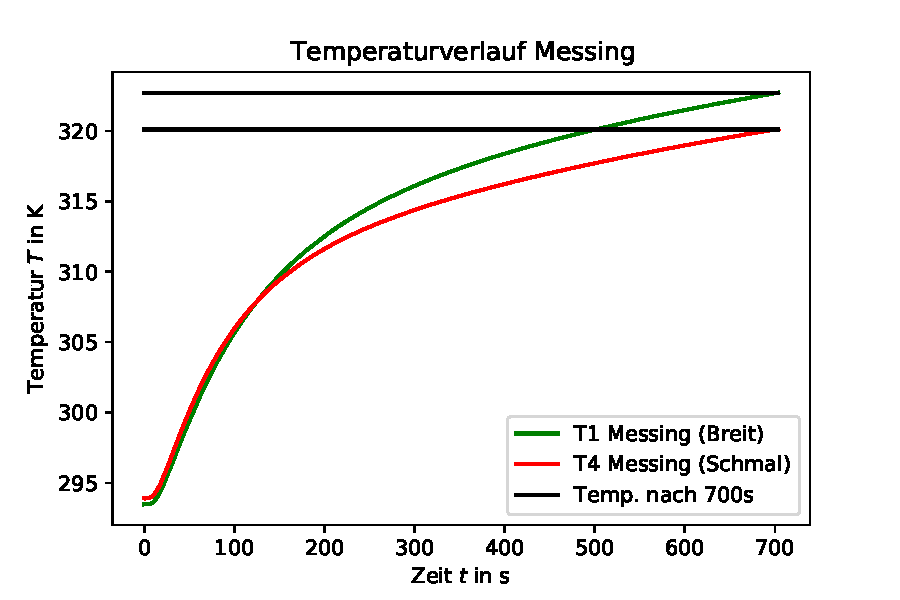
\includegraphics{statmessing.pdf}
    \caption{Statischer Temperaturverlauf von Messing}
    \label{fig:statmess}
  \end{figure}


  \begin{figure}
    \centering
    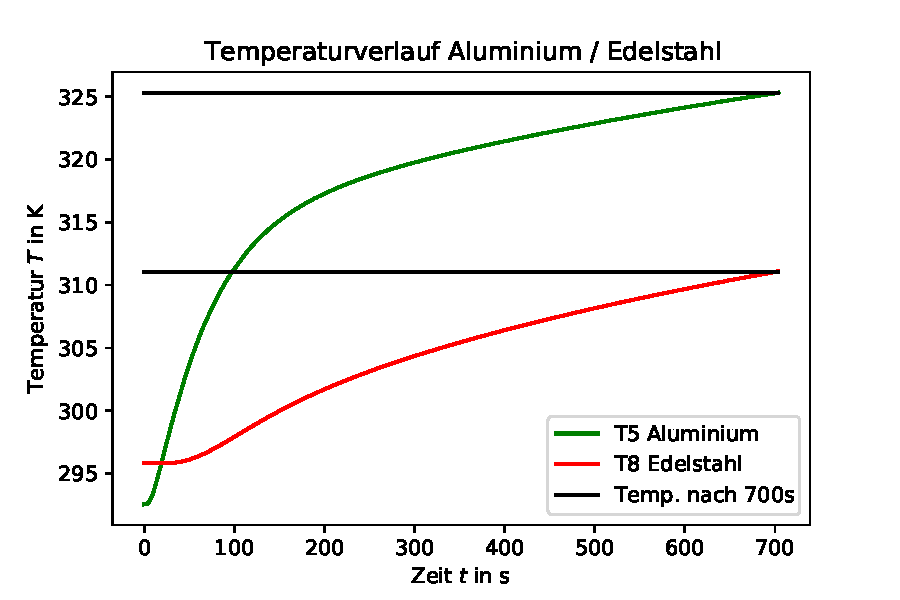
\includegraphics{stataluedel.pdf}
    \caption{Statischer Temperaturverlauf von Messing}
    \label{fig:stataluedel}
  \end{figure}
In \autoref{fig:statmess} und in \autoref{fig:stataluedel} sind die Temperaturverläufe welche an den weiter
vom Heizelement entfernten Temperatursensoren gemessen wurden dargestellt. Zu sehen ist das die Kurven für Messing
am schnellsten ansteigen, die für Aluminium geht bei einer etwas geringeren Temperatur als die Messingkurven 
in ein Plateau über. Der Temperaturverlauf von Edelstahl ist der flachste. Um herauszufinden welcher Metallstab die
beste Wärmeleitung bietet wurden die Temperaturen bei $t=\SI[]{700}[]{s}$ abgelesen, sie sind in
\autoref{tab:siebenhundert} dargestellt. Die höchste Temperatur und damit die beste Wärmeleitfähigkeit hat
demnach Aluminium gefolgt von dem breiten und dem schmalen Messingstab und am Ende dem Edelstahlstab.

  \begin{table}
  \centering
    \caption{Temperatur bei $t=\SI[]{700}[]{s}$}
    \label{tab:siebenhundert}
    \sisetup{table-format=1.2}
    \begin{tabular}{S[table-format=3.2] S S S S S [table-format=3.2]}
      \toprule
      {Thermoelement Nr} & {Temperatur $T$ in K} &{Material}\\
      \midrule
      1 & {$$322.68$$ }&{Messing (breit)} \\
      4 & {$$320.10$$ }&{Messing (schmal)} \\
      5 & {$$325.28$$ }&{Alluminium} \\
      8 & {$$311.04$$ }&{Edelstahl} \\
      \bottomrule
    \end{tabular}
  \end{table}

  Nun wird für verschiedene Zeiten der Wärmestrom $\frac{\Delta Q}{\Delta t}$ bestimmt.
  \begin{table}
    \centering
      \caption{Wärmestrom nach Zeit}
      \label{tab:strom}
      \sisetup{table-format=1.2}
      \begin{tabular}{S[table-format=3.2] S S S S S [table-format=3.2]}
        \toprule
        {Zeitpunkt $t$} &{$(\frac{\Delta Q}{\Delta t})_{Messing breit}$} &{$(\frac{\Delta Q}{\Delta t})_{Messing schmal}$}&{$(\frac{\Delta Q}{\Delta t})_{Aluminium}$}&{$(\frac{\Delta Q}{\Delta t})_{Edelstahl}$}\\
        \midrule
        {$$140.8$$} &{$$0.00927$$}&{$$0.01129$$}&{$$0.00639$$}&{$$0.00600$$} \\
        {$$281.6$$} &{$$0.00570$$}&{$$0.00804$$}&{$$0.00405$$}&{$$0.00545$$} \\
        {$$422.4$$} &{$$0.00468$$}&{$$0.00733$$}&{$$0.00359$$}&{$$0.00511$$} \\
        {$$563.2$$} &{$$0.00439$$}&{$$0.00720$$}&{$$0.00345$$}&{$$0.00493$$} \\
        {$$703.8$$} &{$$0.00432$$}&{$$0.00716$$}&{$$0.00341$$}&{$$0.00483$$} \\
    
        
        \bottomrule
      \end{tabular}
    \end{table}

In \autoref{fig:differenz1} ist die Differenz der beiden Temperatursensoren des Messingstabes
aufgetragen und in \autoref{fig:differenz2} ist die Differenz der Temperatursensorendes Edelstahlstabes  aufgetragen.
Hier fällt auf das der Messingstab die Wärme viel schneller leitet und so die Tepmeraturdifferenz sehr viel schneller
kleiner wird.  
    \begin{figure}
        \centering
        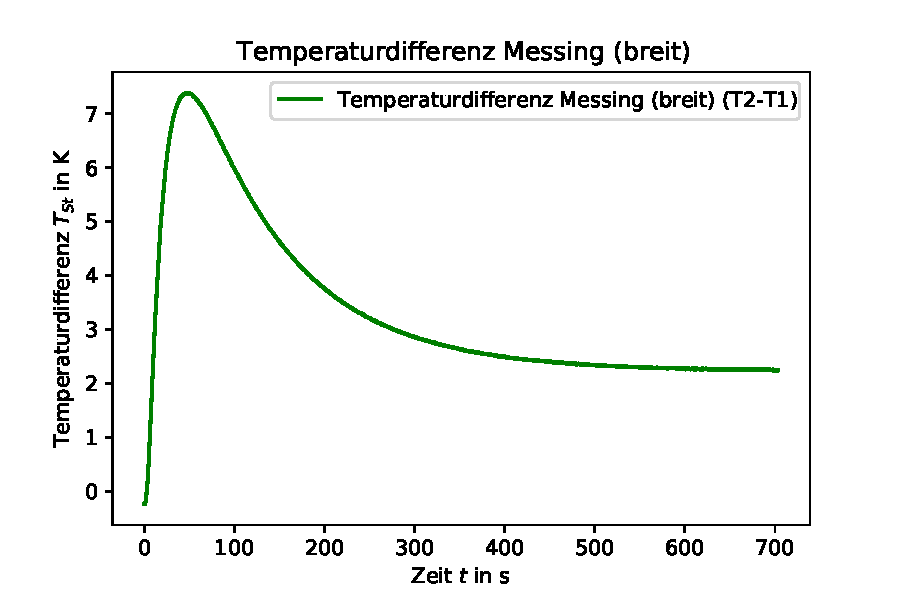
\includegraphics{diffmess.pdf}
        \caption{Temperaturdifferenzverlauf von Messing}
        \label{fig:differenz1}
      \end{figure}
    \begin{figure}
        \centering
        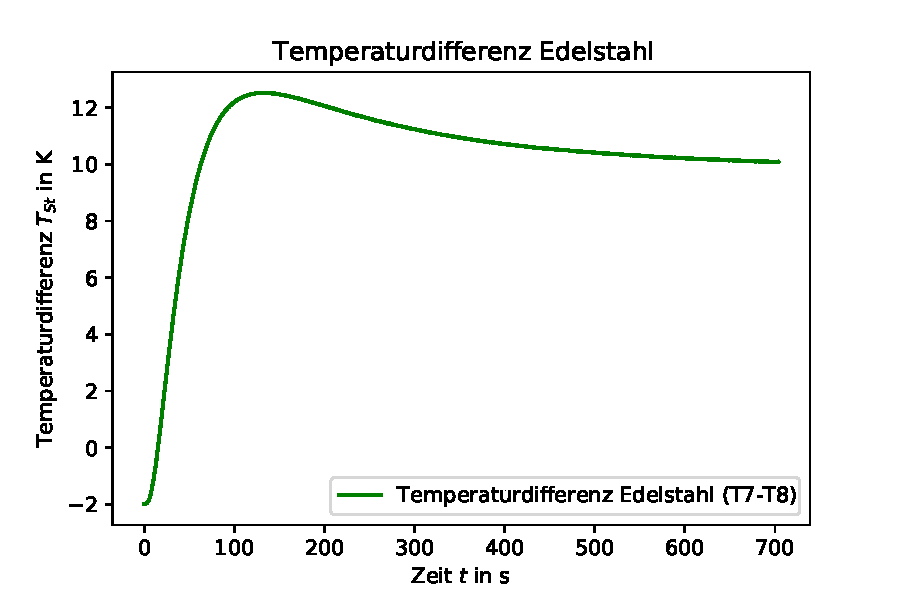
\includegraphics{diffed.pdf}
        \caption{Temperaturdiffernzverlauf von Edelstahl}
        \label{fig:differenz}
      \end{figure}

\subsection{Das Angström Messverfahren}
In diesem Schritt werden die Wärmeleitfähigketen $\kappa$ mit dem Angström Messverfahren also durch
abwechselndes erhitzen und Kühlen der Stäbe genutzt. Dabei wird eine Periodendauer von $T=\SI[]{80}[]{s}$
verwendet. Die Temperaturverläufe sind in \autoref{fig:welmess} für Messing und in \autoref{fig:aluwelle} für Aluminium dargestellt.
\begin{figure}
    \centering
    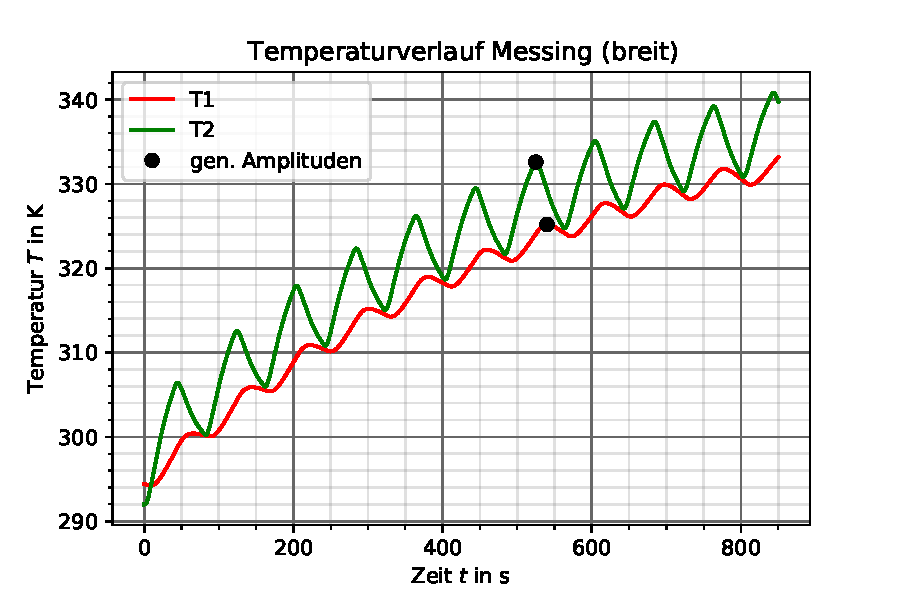
\includegraphics{wellemessing.pdf}
    \caption{Temperaturdiffernzverlauf von Edelstahl}
    \label{fig:wellmess}
  \end{figure}
  \begin{figure}
    \centering
    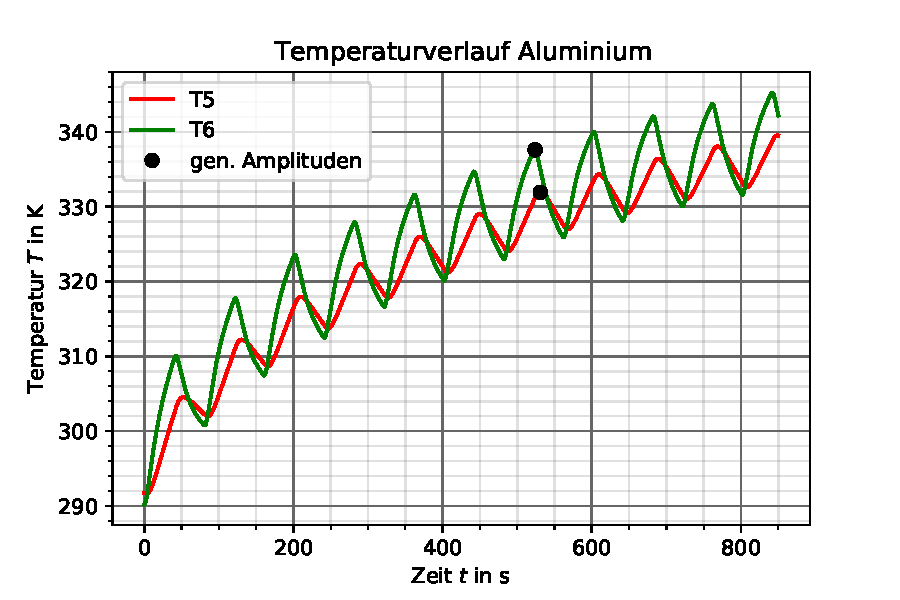
\includegraphics{wellenalu.pdf}
    \caption{Temperaturdiffernzverlauf von Edelstahl}
    \label{fig:aluwelle}
  \end{figure}
  Mit den gekenzeichneten Amplituden folgen sofort die Phasenverschiebungen $\Delta t_{Messing}=\SI[]{15}[]{s}$ 
  und $\Delta t_{Aluminium}=\SI[]{7}[]{s}$, sowie Amplitudenverhältnisse $(\frac{A_{fern}}{A_{nah}})_{Messing}=1.02279$ und $(\frac{A_{fern}}{A_{nah}})_{Aluminium}=1.00800$,
  jetzt lassen sich über \autoref{eq:sechs} sofort die Wärmeleitfähigketen bestimmen:
  \begin{center}
      $\kappa_{Messing}=4367.46\si[]{\frac{W}{K*m}}$\\
      $\kappa_{Aluminium}=18745.14\si[]{\frac{W}{K*m}}$
  \end{center}
  Dazu wurde $\Delta x=\SI[]{0.03}[]{m}$ verwendet.
  Zur Bestimmung von $\kappa_{Edelstahl}$ wurde eine Periodendauer von $T=\SI[]{200}[]{s}$ genutzt \autoref{fig:edelwelle}.
  Die zur bestimmung von $\kappa_{Edelstahl}$ benötigten Amplitudenverhältnisse und Phasendifferenzen
  wurden zuerst einzeln berechnet dann über \autoref{eq:Mittelwert} gemittelt und in \autoref{eq:sechs}
  eingesetzt. Der Fehler des Mittelwertes ergibt sich über \autoref{eq:Mittelwertfehler}, er pflanzt sich bei benutzung
  von \autoref{eq:sechs} über die Gaußsche Fehlerfortpflanzung \autoref{eq:gaussfehler} fort. 
  Das führt zu einem Wert für Edelstahl von:
  \begin{center}
      $\kappa_{Edelstahl}=(-2.3\pm 1.1)\times 10^{4}\si[]{\frac{W}{K*m}}$
  \end{center}
  \begin{figure}
    \centering
    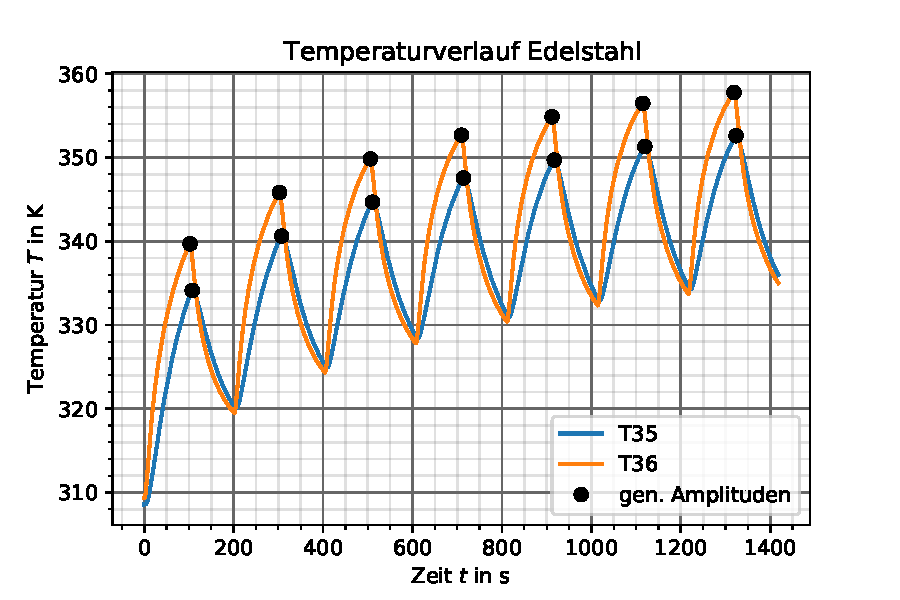
\includegraphics{welleedelstahl.pdf}
    \caption{Temperaturdiffernzverlauf von Edelstahl}
    \label{fig:edelwelle}
  \end{figure}

  Die Wellenlängen und Frequenzen lassen sich einfach bestimmen mit den Zusammenhängen:
  \begin{center}
      $f=\frac{1}{T}$\\
      $v=\frac{\Delta x}{\Delta t}$\\
      $\lambda=\frac{v}{f}$
\end{center}
Daraus folgen sofort die Ergebnisse in \autoref{tab:ergebnisse}.
\begin{table}
    \centering
      \caption{Temperatur bei $t=\SI[]{700}[]{s}$}
      \label{tab:ergebnise}
      \sisetup{table-format=1.2}
      \begin{tabular}{S[table-format=3.2] S S S S S [table-format=3.2]}
        \toprule
        {Material}&{ $T$ / s}&{ $\Delta t$ / s}&{ $v$ / m/s}&{ $f$ / Hz}&{ $\lambda$ / m}\\
        \midrule
        {Messing (breit)}&{$$81$$}&{$$15$$} &{$$0.002$$} &{$$0.0123$$} &{$$0.162$$}  \\
        {Alluminium}&{$$82$$}&{$$7$$} &{$$0.0042$$} &{$$0.0121$$} &{$$0.3471$$} \\
        {Edelstahl}&{$$202.8$$}&{$$4.71$$} &{$$0.00636$$} &{$$0.004932$$} &{$$1.290$$} \\
        \bottomrule
      \end{tabular}
    \end{table}